% Fig. 2 - Legacy RA Procedure (unified style with Fig 3 and Fig 4)
% Compile: pdflatex fig2_legacy_msc.tex
\documentclass[border=5pt]{standalone}
\usepackage{amsmath}
\usepackage{tikz}
\usetikzlibrary{arrows.meta, positioning, calc}

\begin{document}
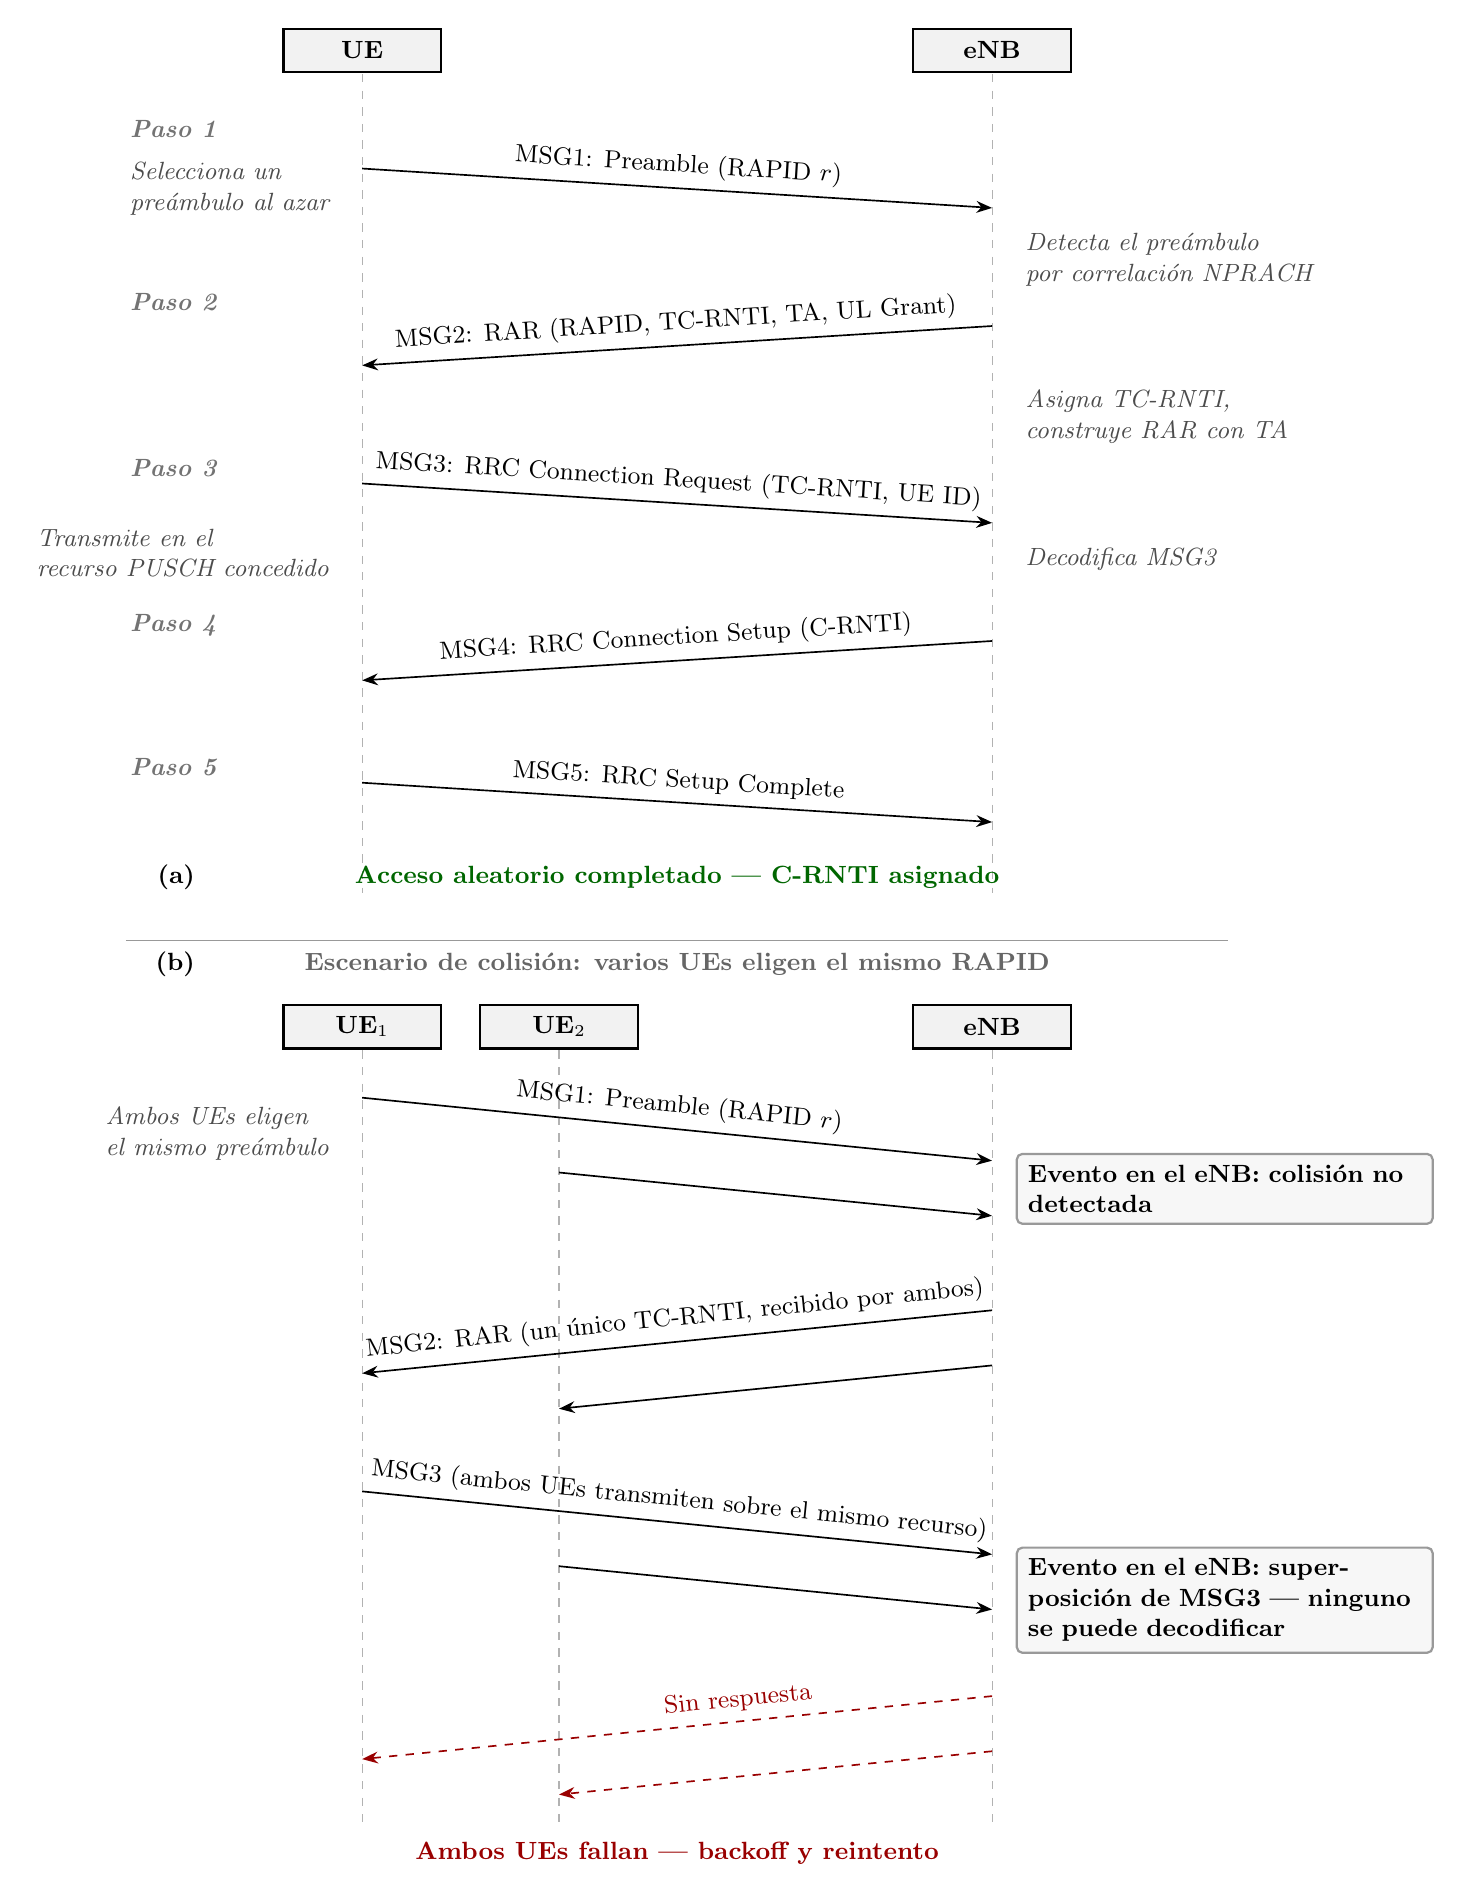
\begin{tikzpicture}[
    >=Stealth,
    font=\small,
    entity/.style={draw, rectangle, minimum width=2cm, minimum height=0.55cm,
                   fill=black!5, font=\small\bfseries, thick},
    msg/.style={->, semithick},
    sidenote/.style={font=\small\itshape, text=black!70, align=left},
    callout/.style={draw=black!40, fill=black!3, rounded corners=2pt,
                    inner sep=4pt, font=\small, align=left, thick=0.4pt,
                    text width=5cm},
    phase/.style={font=\small\bfseries\itshape, text=black!55},
]

% ============================================================
% MAIN FLOW (successful case, single UE)
% ============================================================

% --- Entities ---
\node[entity] (ue) at (0, 0) {UE};
\node[entity] (enb) at (8, 0) {eNB};

% Lifelines
\draw[dashed, black!30, thin] (0, -0.3) -- (0, -10.7);
\draw[dashed, black!30, thin] (8, -0.3) -- (8, -10.7);

% --- Step 1: MSG1 ---
\node[phase] at (-2.4, -1.0) {Paso 1};

\draw[msg] (0, -1.5) -- node[sloped, above, font=\small]
    {MSG1: Preamble (RAPID $r$)} (8, -2.0);

\node[sidenote, anchor=north east] at (-0.3, -1.3)
    {Selecciona un\\preámbulo al azar};

\node[sidenote, anchor=north west] at (8.3, -2.2)
    {Detecta el preámbulo\\por correlación NPRACH};

% --- Step 2: MSG2 ---
\node[phase] at (-2.4, -3.2) {Paso 2};

\draw[msg] (8, -3.5) -- node[sloped, above, font=\small]
    {MSG2: RAR (RAPID, TC-RNTI, TA, UL Grant)} (0, -4.0);

\node[sidenote, anchor=north west] at (8.3, -4.2)
    {Asigna TC-RNTI,\\construye RAR con TA};

% --- Step 3: MSG3 ---
\node[phase] at (-2.4, -5.3) {Paso 3};

\draw[msg] (0, -5.5) -- node[sloped, above, font=\small]
    {MSG3: RRC Connection Request (TC-RNTI, UE ID)} (8, -6.0);

\node[sidenote, anchor=north east] at (-0.3, -5.95)
    {Transmite en el\\recurso PUSCH concedido};

\node[sidenote, anchor=north west] at (8.3, -6.2)
    {Decodifica MSG3};

% --- Step 4: MSG4 ---
\node[phase] at (-2.4, -7.3) {Paso 4};

\draw[msg] (8, -7.5) -- node[sloped, above, font=\small]
    {MSG4: RRC Connection Setup (C-RNTI)} (0, -8.0);

% --- Step 5: MSG5 ---
\node[phase] at (-2.4, -9.1) {Paso 5};

\draw[msg] (0, -9.3) -- node[sloped, above, font=\small]
    {MSG5: RRC Setup Complete} (8, -9.8);

\node[font=\small\bfseries, text=black, anchor=east] at (-2.0, -10.5) {(a)};

\node[font=\small\bfseries, text=green!40!black] at (4, -10.5)
    {Acceso aleatorio completado --- C-RNTI asignado};

% ============================================================
% SEPARATOR
% ============================================================
\draw[thin, black!40] (-3, -11.3) -- (11, -11.3);
\node[font=\small\bfseries, text=black, anchor=east] at (-2.0, -11.6) {(b)};
\node[font=\small\bfseries, text=black!60] at (4, -11.6)
    {Escenario de colisión: varios UEs eligen el mismo RAPID};

% ============================================================
% COLLISION SUB-SCENARIO (unified style: black solid msgs, gray lifelines)
% ============================================================

% Sub-entities (same style and spacing as Fig 3/4: UE1=0, UE2=2.5, eNB=8)
\node[entity] (ue1c) at (0, -12.4) {UE$_1$};
\node[entity] (ue2c) at (2.5, -12.4) {UE$_2$};
\node[entity] (enbc) at (8, -12.4) {eNB};

% Sub-lifelines (gray dashed, extended)
\draw[dashed, black!30, thin] (0, -12.7) -- (0, -22.5);
\draw[dashed, black!30, thin] (2.5, -12.7) -- (2.5, -22.5);
\draw[dashed, black!30, thin] (8, -12.7) -- (8, -22.5);

% ============================================================
% Collision MSG1 (parallel, slope -0.1, y-intercept spacing 0.7)
% UE1: (0,-13.3) → (8,-14.1)
% UE2: (2.5,-14.25) → (8,-14.8)
% ============================================================
\draw[msg] (0, -13.3) -- node[sloped, above, font=\small, pos=0.5]
    {MSG1: Preamble (RAPID $r$)} (8, -14.1);
\draw[msg] (2.5, -14.25) -- (8, -14.8);

\node[sidenote, anchor=north east] at (-0.3, -13.3)
    {Ambos UEs eligen\\el mismo preámbulo};

\node[callout, anchor=north west] at (8.3, -14.0) {
    \textbf{Evento en el eNB: colisión no detectada}
};

% ============================================================
% Fallback RAR (eNB → both UEs, parallel, slope +0.1, spacing 0.7)
% Arrow to UE1: (8,-16.0) → (0,-16.8)
% Arrow to UE2: (8,-16.7) → (2.5,-17.25)
% ============================================================
\draw[msg] (8, -16.0) -- node[sloped, above, font=\small, pos=0.5]
    {MSG2: RAR (un único TC-RNTI, recibido por ambos)} (0, -16.8);
\draw[msg] (8, -16.7) -- (2.5, -17.25);

% ============================================================
% MSG3 from both UEs (parallel, slope -0.1, spacing 0.7)
% UE1: (0,-18.3) → (8,-19.1)
% UE2: (2.5,-19.25) → (8,-19.8)
% ============================================================
\draw[msg] (0, -18.3) -- node[sloped, above, font=\small, pos=0.5]
    {MSG3 (ambos UEs transmiten sobre el mismo recurso)} (8, -19.1);
\draw[msg] (2.5, -19.25) -- (8, -19.8);

\node[callout, anchor=north west] at (8.3, -19.0) {
    \textbf{Evento en el eNB: superposición de MSG3 --- ninguno se puede decodificar}
};

% Failure outcome (no MSG4 sent; red dashed to both UEs, parallel)
% To UE1: (8,-20.9) → (0,-21.7),   To UE2: (8,-21.6) → (2.5,-22.15)
\draw[->, semithick, red!60!black, dashed] (8, -20.9) --
    node[sloped, above, font=\small, text=red!60!black, pos=0.4]
    {Sin respuesta} (0, -21.7);
\draw[->, semithick, red!60!black, dashed] (8, -21.6) -- (2.5, -22.15);

\node[font=\small\bfseries, text=red!60!black] at (4, -22.9)
    {Ambos UEs fallan --- backoff y reintento};

\end{tikzpicture}
\end{document}
